\documentclass{article}
\usepackage{gset}
\usepackage{preamble}

\begin{document}
	\maintitle{Матан Дз 5}
	\textbf{1)}  \bs a)
	Опишем обход числовой плоскости. Начнем из точки (0,0) - эта пара будет соответствовать числу 1. Затем сделаем шаг в положительном направлении оси Х, затем как по квадрату обойдем точки с целыми координатами по часовой стрелке, повторим процесс. Таким образом, каждому натуральному числу будет соответствовать ровно одна пара из целых чисел. Нагляднее показать на картинке. \bs
	\[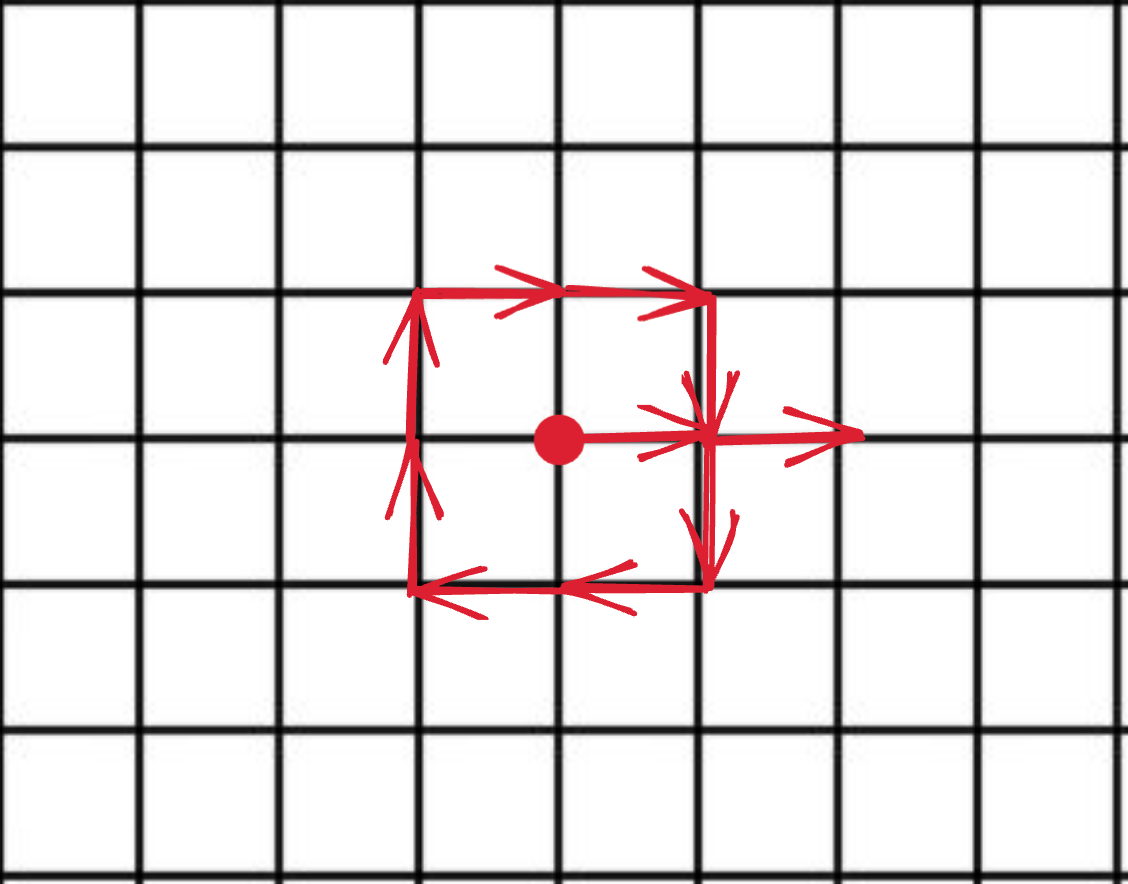
\includegraphics[width=75mm]{img}\]
	\bs
	b) Мы можем расселить все рациональные числа как на картинке (по аналогии с парадоском отеля), при этом 0 переставим на место 1. Иррациональные числа оставим на месте, потому что их количество не меняется. 
	\[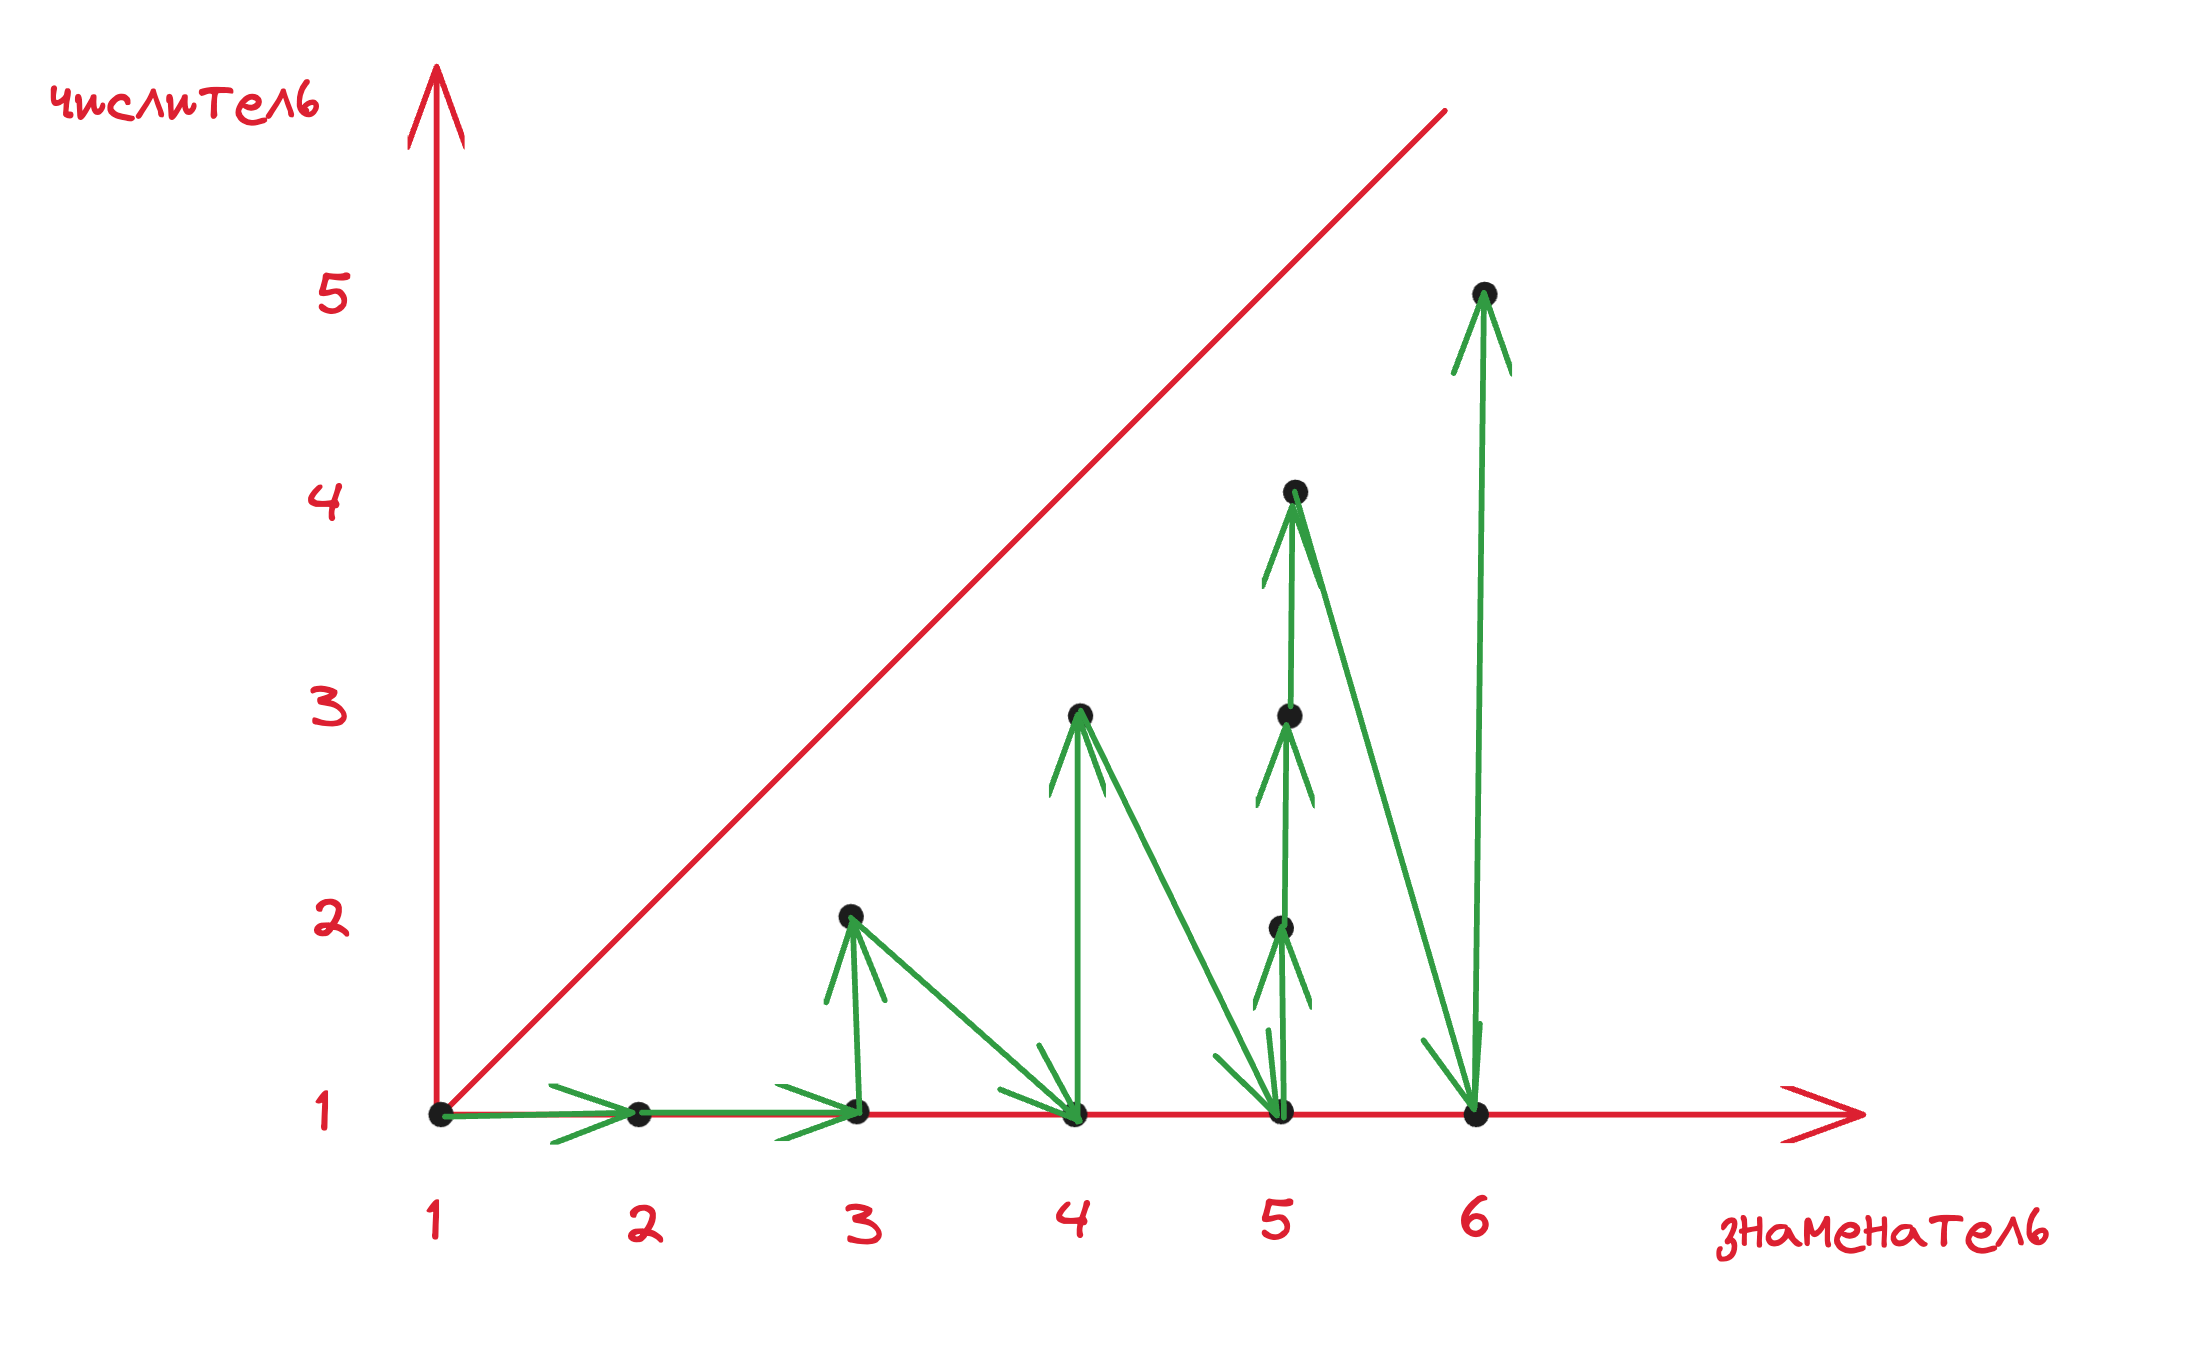
\includegraphics[width=100mm]{img2}\]
	\bs
	\textbf{2)}  \bs
	a) Пусть $a_k = (-1)^k, b_k = (-1)^{k + 1}$ \sspace
	$\overline{\lim\limits_{k\to \infty}} a_k = \overline{\lim\limits_{k\to \infty}} b_{k} = 1 \quad \overline{\lim\limits_{k\to \infty}} a_k*b_k = -1$ \sspace
	$
	-1 < 1 * 1 \sspace
	$
	b) Пусть $a_k = b_k = (-1)^{k + 1}$ \sspace
	$
	\underline{\lim\limits_{k\to \infty}} a_k = \underline{\lim\limits_{k\to \infty}} b_k = -1 \quad \underline{\lim\limits_{k\to \infty}} a_k  + b_k  = 0 \sspace
	-1 -1 < 0
	$
	\sspace
	c) Пусть $a_k = -1, b_k = (-2)^k$ \sspace
	$
	\lim\limits_{k\to \infty} a_k = -1 \quad \overline{\lim\limits_{k\to \infty}} a_k * b_k =  2 \quad -1 * \overline{\lim\limits_{k\to \infty}} b_k = -1 * 2 = -2
	\sspace
	-2 \neq 2
	$ \bs
	\textbf{3)}\bs
	a) $a_k = \dfrac{{(-1)}^k}{k} + \dfrac{1 + (-1)^k}{2}$ \sspace
	$\overline{\lim\limits_{k\to \infty}} a_k = 1 \quad \underline{\lim\limits_{k\to \infty}} a_k = 0 \quad \sup{\{a_k\}}_{k=1}^{+\infty} = a_2 = \dfrac{3}{2}  \quad \inf{\{a_k\}}_{k = 1}^{+\infty} = a_1 = -1 \bs$
	b) $a_k = \dfrac{((-1)^k - 1)k^2 + k + 1}{k} \sspace$ 
	$\forall k = 2n, n \in \mathbb{N} \hookrightarrow a_k = \dfrac{k + 1}{k}  = b_k \sspace
	\forall k = 2n - 1, n \in \mathbb{N} \hookrightarrow a_k = \dfrac{-2k^2 + k + 1}{k} = -2k + 1 - \dfrac{1}{k} = c_k \sspace
	\lim\limits_{n\to \infty} b_k = 1 \quad \lim\limits_{k\to \infty} c_n = -\infty \sspace
	\overline{\lim\limits_{k\to \infty}} a_k = 1 \quad \underline{\lim\limits_{k\to \infty}} a_k = -\infty \quad \sup{\{a_k\}}_{k=1}^{+\infty} = a_2 = \dfrac{3}{2}  \quad \inf{\{a_k\}}_{k = 1}^{+\infty} = -\infty \bs
	$ 
	c) $a_k = 1 + 2(-1)^{k + 1} + 3(-1)^{\frac{k(k - 1)}{2}} \sspace
	$
	\[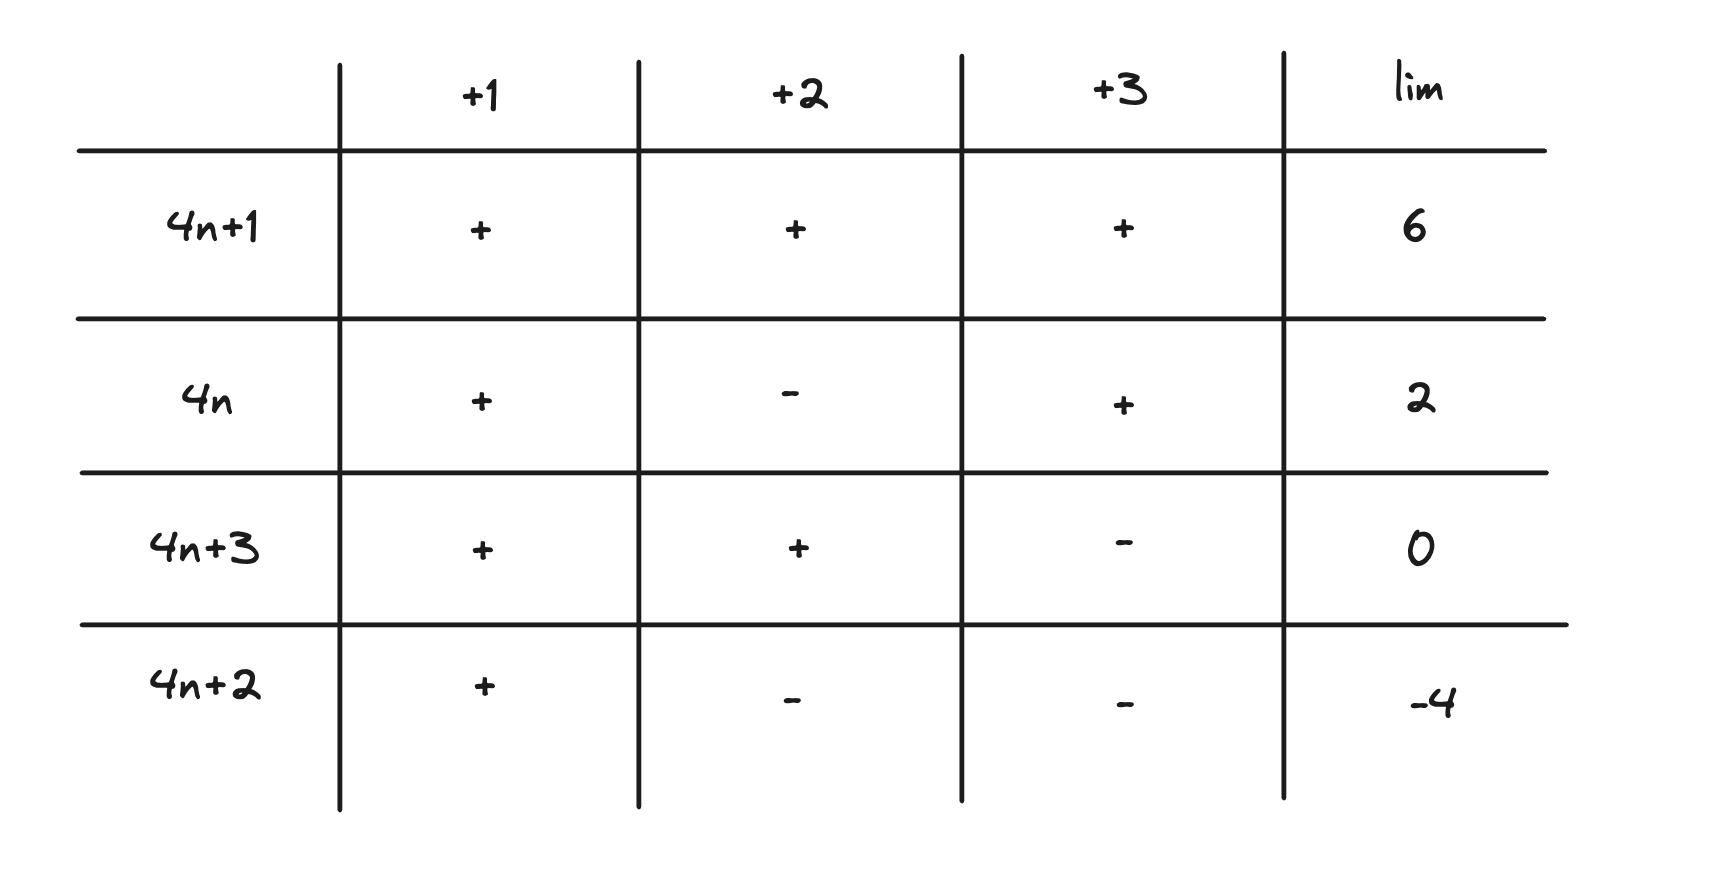
\includegraphics[width=150mm]{img3}\] \bs
	Можно разбить свю последовательность на 4 подпоследовательности, пределы которых будут 6, 4, 3, 1, как в таблице. Соответственно получим \sspace
	$\overline{\lim\limits_{k\to \infty}} a_k = 6 \quad \underline{\lim\limits_{k\to \infty}} a_k = -4 \quad \sup{\{a_k\}}_{k=1}^{+\infty} = 6  \quad \inf{\{a_k\}}_{k = 1}^{+\infty} = -4 \bs$
	\textbf{4)} \bs
	a) $\sum_{k=1}^{\infty} \bigg\{\dfrac{1}{\sqrt{k + 1} + \sqrt{k}} =  \dfrac{\sqrt{k + 1} - \sqrt{k}}{1}\bigg\} = \infty$ \sspace
	Раскрываем как телескопическую сумму, остается только первый и последний член, тк последний член бесконечность, то и вся сумма тоже бесконечность \sspace
	b) $\sum_{k = 1}^{\infty} \{\cos{kx}\}$ \sspace
	Предположим, что все элементы ряда 0, тогда $kx = \dfrac{(2n - 1)\pi}{2}, n \in \mathbb{N} \Rightarrow x = \dfrac{(2n - 1)\pi}{2k}$ \sspace Это значит, что x зависит от k, хотя не должен. Получается, что для каждого k нужен свой х, но так как х одинаковый при всех k, то такой случай невозможен. \sspace
	Получается, что в ряду есть ненулевые элементы, будем дальше рассматривать только их, потому что нулевые не влияют на сумму. \sspace
	Пусть $\exists a \in \mathbb{R}: \sum_{k = 1}^{\infty} \cos(kx)= a \lra \sum_{k = 1}^{\infty} \cos{((k + 1) * x)}= a \Rightarrow \lim\limits_{n \to \infty} (kx + x) = 0$ \sspace
	1 переход, потому что если ряд сходится, то если отбросить его первые сколько-то элементов, он продолжит сходиться. 2 переход, потому что если ряд сходится, то его общий член стремится к 0. \sspace
	Пусть это верно
	$
	\lim\limits_{n \to \infty} \cos(kx + x) = 0 \lra \lim\limits_{n \to \infty} \cos(kx) * \cos x - \sin(kx) * \sin x = 0 \lra \lim\limits_{n \to \infty} \sin(kx) * \sin x = 0 \lra \lim\limits_{n \to \infty} \sin(kx) = 0 \sspace
	$ 
	Последний переход, потому что $\sin x$ константа. Получаем противоречие, потому что по основному тригонометрическому тождеству $\sin^2 x + \cos^2 x = 1$. Значит предположение неверно, значит ряд расходится
\end{document}